\chapter{Future Explorations and Wreath-building Dynamos with Tachoclines}
\label{chapter:the promise of the future}
In this thesis we have explored a variety of dynamo solutions in stars
rotating more rapidly than the sun.  Magnetic wreaths arise as a near
ubiquitous feature of these simulations, irrespective of rotation rate
or level of turbulence achieved.  These simulations have at present
included the convection zone only.  In many solar dynamo theories,
it is thought that the tachocline must play a major role.  Clearly, a
major thrust of future research must be the inclusion of this
important internal boundary layer.  

In studies of compressible convection that include regions of
penetration at the bottom of the convection zone, organized magnetic
fields are often efficiently pumped downwards and out of the
convection zone \citep[e.g.,][]{Tobias_et_al_2001,
  Browning_et_al_2006}.  Magnetic wreaths might be efficiently
expelled from the convection zone by the compressible convection
there.  This could remove them from the region of amplification, as
the poloidal field may not be regenerated within the tachocline by the
same processes at work within the convection zone.  This would
likely cause magnetic wreaths to vanish entirely.  Such a finding
would cast serious doubt on the viability of magnetic wreaths in turbulent
stellar convection zones.

We have begun explorations into whether magnetic wreaths survive in
the presence of a tachocline in rapidly rotating suns.  We find that
the wreaths do survive, and indeed continue to fill the bulk of the
convection zone, even as they become rooted within the tachocline.
These wreaths still undergo temporal oscillations and cycles of
polarity reversal.  Preliminary results are reported on
here for one simulation rotating at three times the solar rate,
case~T3, with similar input parameters to our wreath building
case~D3. 

\section{Capturing a Model Tachocline within ASH}
The primary parameters of case~T3 are reported in Table~\ref{table:case
  T3} and are similar to our cases~D3 and D3a.  Case~T3 has a lower
boundary at $r=0.5\:R_\odot$ and an upper boundary at
$0.965\:R_\odot$.  There is thus an overall
density contrast of 48 across the convection zone and 133 
across the entire shell.  This leads to somewhat lower values of
$\nu$, $\kappa$ and $\eta$ than in case~D3, despite the two
cases sharing the same values for eddy diffusivities at the top of the
convection zone.   

After thousands of days of
evolution, this dynamo establishes a stable profile of
$\mathrm{d}\bar{S}/\mathrm{d}r$, with the base of the convection zone
where $\mathrm{d}\bar{S}/\mathrm{d}r$ crosses zero located at
approximately $0.705\: R_\odot$.  The fluctuating radial velocities
extend somewhat deeper, and decrease from an average amplitude
of $25\: \mathrm{m}\: \mathrm{s}^{-1}$ to about $1\: \mathrm{m}\:
\mathrm{s}^{-1}$ by a depth of approximately $0.66\: R_\odot$.  The
fluctuating radial flows are much smaller below this
depth.  The peak downflows are moving at almost $-200\:
\mathrm{m}\: \mathrm{s}^{-1}$ at $0.705\: R_\odot$ but have slowed to
roughly $-10\: \mathrm{m}\: \mathrm{s}^{-1}$ when they reach $0.66\: R_\odot$.



\begin{deluxetable}{cccccccccrc}
%\rotatedeluxetable
   \tabletypesize{\footnotesize}
    \tablecolumns{11}
    \tablewidth{0pt}  % `natural' size 
    \tablecaption{Parameters of case~T3
    \label{table:case T3}}
    \tablehead{\colhead{$N_r,N_\theta,N_\phi$} &
      \colhead{Ra} &
      \colhead{Ta} &
      \colhead{Re} &
      \colhead{Re$'$} &
      \colhead{Rm} &
      \colhead{Rm$'$} &
      \colhead{Ro} &
      \colhead{Roc} &
      \colhead{$\nu$} &
      \colhead{$\eta$} 
   }
   \startdata
   $ 258 \times  256 \times  512$ &    9.64$ \times 10^{  5}$ &     1.39$ \times 10^{  7}$ & 184 &  129 &   92 &   64 &    0.481 &    0.333 &     1.37 &     2.75\\
 \enddata
 \tablecomments{Simulation parameters for case~T3 rotating at $3\:
   \Omega_\odot$ and with a tachocline of shear.	Parameters
   have same definition as in
   Table~\ref{table:pm0.5_dynamos_sim_parameters}, with a deep inner
   radius of  $r_\mathrm{bot} = 3.8 \times 10^{10}$cm and outer radius of 
   $r_\mathrm{top} = 6.72 \times 10^{10}$cm.  The base of convection
   zone is at $r_\mathrm{bcz} = 4.91 \times 10^{10}$cm or $0.705\:
   R_\odot$.  Here we define $L = (r_\mathrm{top}-r_\mathrm{bcz}) =
   1.81 \times 10^{10}$cm or $0.26\: R_\odot$.}
\end{deluxetable}

\clearpage
To prevent the diffusive spread of the differential rotation profile
from the convection zone into the stable radiative zone, we taper our
eddy diffusivities with a smooth step function 
\begin{equation}
     \nu(r)  = \nu_0 \left(\frac{\bar{\rho}_0}{\bar{\rho}(r)}\right)^\alpha \Phi(r)\:,
     \quad % \quad
     \kappa(r)  = \kappa_0 \left(\frac{\bar{\rho}_0}{\bar{\rho}(r)}\right)^\alpha \Phi(r)\:,
     \quad % \quad
     \eta(r)  = \eta_0 \left(\frac{\bar{\rho}_0}{\bar{\rho}(r)}\right)^\alpha \Phi(r)\:,
\end{equation}
where $\alpha=-0.5$ as before, $\nu_0$, $\kappa_0$ and $\eta_0$ are the values
at the top of the convection zone and our taper with radius is given by
\begin{equation}
  \Phi(r) = \frac{1}{2} \left(1 - \beta\right)
  \left( 1 + \tanh{\left(\frac{r - r_\mathrm{taper}}{\Delta_\mathrm{taper}}\right)}\right) +\beta\:.
\end{equation}
We recover our treatment of eddy diffusivities in the convection-zone
dynamos when $\Phi=1$ at all radii.
In case~T3 the taper function is centered at $r_\mathrm{taper}=4.70
\times 10^{10}\:$cm ($0.675\:R_\odot$) with width
$\Delta_\mathrm{taper}=5 \times 10^{8}\:$cm ($0.007\:R_\odot$).
The variable $\beta$ controls the amplitude of the tapering function,
which ranges from a value of one in the convection zone to $\beta$ in
the radiative interior.  Here we set $\beta=10^{-2}$ thus reducing our
eddy diffusivities by two orders of magnitude in the stable radiative interior.

We expect that turbulent mixing and transport should
generally be lower in the stable radiative zone than in the unstable
convection zone, but these eddy diffusivities are still many orders of
magnitude larger than the microscopic viscosities and diffusivities
present in stellar interiors.  Over long intervals of time, the
differential rotation will still diffusively spread into the radiative
interior.  By tapering our eddy diffusivities by two orders of
magnitude, we find that the differential rotation produced by
convection remains well confined to the convection zone for more than
7000~days. It is likely that artificially lowering our
viscosities is a more physically plausible approach to preventing
``tachocline-creep'' than other techniques employed in the
past, which included mechanical forcing in the radiative zone and
entropy forcing in the region of the tachocline to retain a comparably
good structure of differential rotation
\citep[e.g.,][]{Browning_et_al_2006}.  

\clearpage
\begin{figure}[!t]
  \begin{center}
    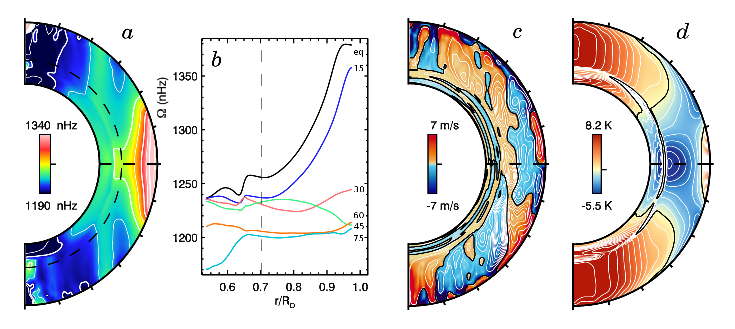
\includegraphics{figs/chapter_9/case_T3_mean_flows.eps}
  \end{center}
  \caption[Profiles of mean flows and temperature in dynamo case~T3]
          {Profiles of mean flows and temperature in dynamo case~T3.
            These profiles are averaged over the interval from
            days~4050-4150 of dynamo case~T3.  The hydrodynamic
            progenitor ran for an additional 600 days previous to day~0.
            $(a)$~Profile of differential rotation
            $\Omega$ with $(b)$~accompanying radial cuts at selected
            latitudes as labeled.  The bottom
            of the convection zone at $r_\mathrm{bcz}=0.705\:R_\odot$
            is marked on both with a dashed line.  The equator is
            prograde, the poles are retrograde and the radiative
            interior is in nearly solid-body rotation between
            latitudes $\pm45^\circ$.
            $(c)$~Meridional circulations with surface structure and
            amplitudes similar to those in case~D3 but different at
            depth.  $(d)$~Profile of latitudinal temperature
            variations relative to the spherically symmetric average $\bar{T}$.
            \label{fig:T3 mean flows}}
          \vskip-0.5cm
\end{figure}

Time-averaged profiles of the differential rotation, meridional
circulations and latitudinal temperature variations of case~T3 are shown in
Figure~\ref{fig:T3 mean flows}.  After a total of more than 4500~days of 
evolution in both the hydrodynamic progenitor and then in case~T3, the
differential rotation remains well confined to the convection zone
(Fig.~\ref{fig:T3 mean flows}$a$).
Within the convection zone, there is a significant angular velocity
contrast in latitude and radius, with a $\Delta \Omega_\mathrm{lat}$
near the surface of $1.04 \thinspace\mu \mathrm{rad}\: s^{-1}$ and
a $\Delta \Omega_r$ across the convection zone at the equator of
$0.89 \thinspace\mu \mathrm{rad}\: s^{-1}$.  The latitudinal angular
velocity contrast is similar to that achieved in dynamo case~D3b, but
the radial contrast is somewhat larger.  Below the base of the
convection zone, the location of the eddy diffusivity taper is visible
as a slight contour in the profile of $\Omega$ (Fig.~\ref{fig:T3 mean
 flows}$a$) and as a small kink in the radial cuts of the same
(Fig.~\ref{fig:T3 mean flows}$b$).  In the radiative interior, a small
latitudinal angular velocity contrast persists.  This is especially
prominent in the polar regions at latitudes above~$\pm60^\circ$.  Near
the equator and up to latitudes of roughly $\pm45^\circ$
the radiative interior is almost in solid-body rotation.

The meridional circulations achieved in case~T3
are shown in Figure~\ref{fig:T3 mean flows}$c$.  In the upper
convection zone, these circulations are similar to those found in
case~D3 (e.g., Fig.~\ref{fig:case_D3_patterns}$d$).  In the lower
convection zone the flows penetrate into the tachocline and radiative
interior.  This largely removes the narrow return flow seen at the
base of case~D3 from the convection zone.  The latitudinal temperature
variations achieved in case~T3 are shown in Figure~\ref{fig:T3 mean
  flows}$c$.  As in the other rapidly rotating simulations, the
convection builds a prominent gradient in latitude, with hot
poles, cool mid-latitudes and a warm equator near the surface.  The
temperature gradients appear to have spread into the radiative interior, and
the thermal wind associated with this likely helps maintain the small
differential rotation that is present there.  Temperature gradients
will diffusively spread more easily than gradients in angular
velocity, owing to the low Prandtl number of this simulation (as
before, $\mathrm{Pr}=0.25$). Lowering the value of $\beta$ in the
tapering function would likely further curtail this spreading, as
would reducing $\nu$ and $\kappa$ throughout the convection zone. 

\section{Magnetic Wreathes with a Tachocline}
\label{sec:tachocline}

Case~T3 continues to build large wreaths of magnetism that fill the
bulk of its convection zone.  The time history of this case is shown
in Figure~\ref{fig:T3}.  As in many of our other rapidly rotating
dynamos, wreaths appear at latitudes of roughly $\pm20^\circ$ and undergo cycles of
polarity change.  In the 5800 days shown here, four polarity reversals
occur in both hemispheres after the dynamo saturates at roughly
day~1000.  The wreaths are strong at mid-convection zone and stronger
yet near the base of the convection zone (Figs.~\ref{fig:T3}$c,d$).    
\begin{figure}
  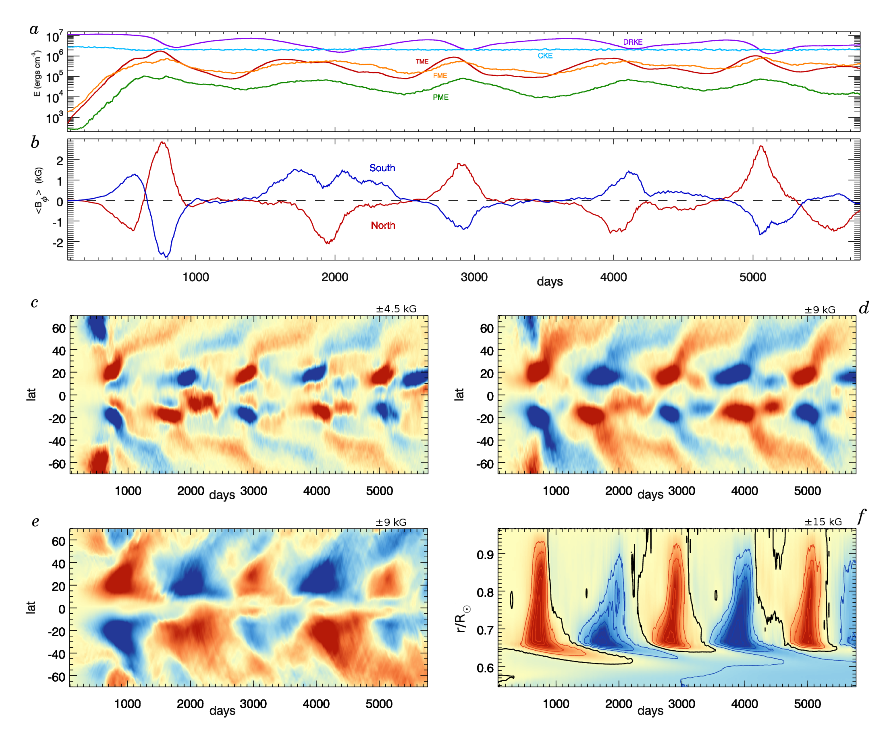
\includegraphics{figs/chapter_9/mhd_tacho_3_time_history.eps}
  % note: scaled to 145 mm width before saving to eps; original file is
  % unscaled (~180 mm width)
  \caption[Time-dependent behavior in case~T3 with a model tachocline]
	  {Time-dependent behavior in case~T3 with a model tachocline.  
          $(a)$~Volume-averaged kinetic and magnetic energies, and
            $(b)$~mean $\langle B_\phi \rangle$ averaged over northern
            and southern hemispheres at mid-convection zone.  
            $(c)$~Time-latitude maps of $\langle B_\phi \rangle$ at
            mid-convection zone ($0.85\: R_\odot$) and $(d)$~near the
            base of the convection zone ($0.7\: R_\odot$).  Multiple
            cycles of wreath building occur in the roughly 5000~days
            after dynamo saturation.  $(e)$~The~wreaths extend into
            the tachocline ($0.65\: R_\odot$), with somewhat broader
            structure.  At greater depths single polarity wreaths
            persist for the entire simulated interval.  
            $(f)$~Time-radius map at a fixed latitude of $20^\circ$, in the
            core of the northern hemisphere wreaths.  The black
            contour denotes the neutral line between successive
            wreaths. 
          \label{fig:T3}}
\end{figure}
In both regions the wreaths have similar latitudinal structure.
In the tachocline, the wreaths occupy a broader range of latitudes and
remain strong  (Fig.~\ref{fig:T3}$e$).  Time-radius maps at a fixed latitude of $20^\circ$, in
the core of the magnetic wreaths, show that with each successive
polarity reversal some field of the previous cycle migrates deeper
into the radiative interior (Fig.~\ref{fig:T3}$f$).  At depths below $0.6\: R_\odot$ however
a single polarity of wreathes are established and persist.  During the
5800~days shown here, these deep magnetic structures slowly grow in
strength.  By the end of this interval, the mean toroidal fields have reached
peak amplitudes of nearly $\pm 9\:$kG near the bottom boundary, with
the strongest fields appearing near latitudes of $\pm55^\circ$.  These deep
fields may  arise from turbulent transport and pumping within the
convection zone and coupled down into the deep radiative interior.
It seems more likely however that they result from stretching of the initial
weak seed field by the differential rotation that has diffusively spread into
the polar regions of the radiative interior, as the peak angular
velocity contrast there occurs at the higher latitudes where the
wreaths are located.  Decreasing our tapering constant
$\beta$ to values of $10^{-3}$ or less should strongly decrease the
diffusive spread of differential rotation and suppress the generation
of these deep-seated wreaths.








\begin{figure}[!t]
  \begin{center}
    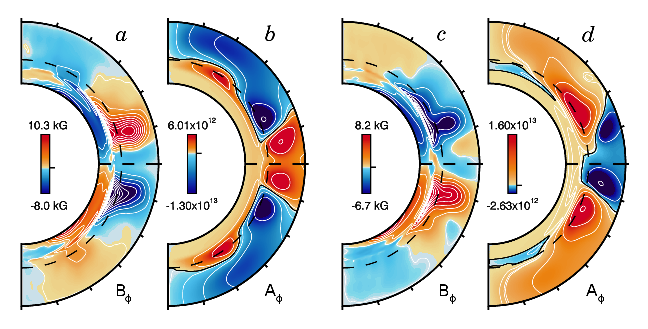
\includegraphics{figs/chapter_9/mhd_tacho_3_mean_fields.eps}
  \end{center}
  \caption[Profiles of $\langle B_\phi \rangle$ and $\langle A_\phi \rangle$ in dynamo case~T3]
          {Profiles of $\langle B_\phi \rangle$ and $\langle A_\phi \rangle$ in dynamo case~T3.
          $(a)$~Mean toroidal magnetic field $\langle B_\phi \rangle$ and
            $(b)$~poloidal vector potential $\langle A_\phi \rangle$ 
            averaged over days~4050-4150 at a time of peak
            mean fields.  At this time, the
            wreaths and associated mean-poloidal field are out of phase
            with the magnetic field in the deep interior.
          $(d)$~$\langle B_\phi \rangle$ and $(e)$ $\langle A_\phi \rangle$
            averaged over days~5000-5100 when the fields have flipped
            polarity and again reached peak amplitudes.  At this time,
            the magnetic fields in the convection zone have the same
            polarity as those in the radiative interior.  The bottom
            of the convection zone at $r_\mathrm{bcz}=0.705\:R_\odot$ is
            indicated by the dashed semi-circle.
          \label{fig:T3 mean fields}}
\end{figure}

Time-averaged profiles of the mean toroidal fields and poloidal vector
potential are shown at two intervals in Figure~\ref{fig:T3 mean
  fields}.  At both times the wreaths of magnetism are at a point in
the cycles of polarity reversal where the fields have attained peak
amplitudes.  The mean magnetic fields associated with the wreaths 
extend into the tachocline down to roughly where the eddy
diffusivities taper in amplitude.   This depth also roughly
coincides with the depth at which the fastest downflows have their 
motion substantially braked by the stable stratification.


The mean fields produced in the convection zone undergo cycles of
polarity reversal, while those deep in the radiative interior always
retain the same polarity. During the first cycle shown in
Figure~\ref{fig:T3 mean fields}, spanning days 4050-4150, the
mean magnetic fields in the convection zone have opposite polarity
from the fields in the radiative interior (Figs.~\ref{fig:T3 mean fields}$a,b$).  
After the fields flip in polarity and regrow in amplitude, they match
the polarity of the radiative interior fields (days~5050-5150;
Figs.~\ref{fig:T3 mean fields}$c,d$).   At present, it is unclear
whether the dynamo behaves substantially differently when the
convection either matches or opposes the fields in the radiative
interior.  Convective patterns and the global-scale flows of
differential rotation and meridional circulation are very similar
during both of the intervals examined here.


These simulations of dynamo action in the presence of a tachocline are
very promising.  Wreaths of magnetism continue to fill the bulk of the
convection zone and undergo cycles of polarity reversal.  These
polarity reversals occur on similar timescales to those found in the
convection-zone dynamos studied in Chapters~\ref{chapter:case D5} and
\ref{chapter:menagerie of dynamos}.  The polarity reversals in real
stars generally have slightly longer periods than those found here,
and in the Sun magnetic polarity reversals occur on a time scale of
roughly 11~years, or about 4000~days.  



\begin{figure}[!t]
  \begin{center}
    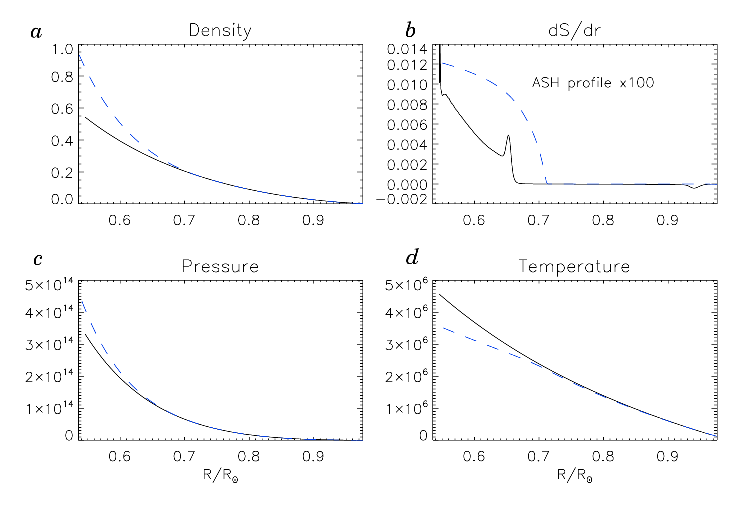
\includegraphics{figs/chapter_9/mhd_tacho_3_structure.eps}
  \end{center}
  \caption[Stellar structure of case~T3]
          {Stellar structure of case~T3.  Shown are spherically
            symmetric profiles of thermodynamic variables 
            $(a)$~$\bar{\rho}$, $(b)$~$\mathrm{d}\bar{S}/\mathrm{d}r$,
            $(c)$~$\bar{P}$ and $(d)$~$\bar{T}$.   
            The adopted structure in ASH is shown with a black, solid
            line and the CESAM solar structure model is shown with a
            blue, dashed line \citep[from][]{Brun_et_al_2002}.  The
            ASH entropy gradient shown in $(b)$ has been multiplied by
            a factor of 100 to make it visible.  The
            ASH structure and solar model are in good agreement within
            the convection zone, but diverge in the radiative
            interior.
            \label{fig:T3 structure}}
\end{figure}

Our dynamo with a tachocline shows promise, but the model could be
improved significantly.  The background structure used within case~T3
is shown in Figure~\ref{fig:T3 structure}.  
At present, our thermodynamic variables are in decent agreement with
the solar structure model \citep[a CESAM model based on work
  in][]{Brun_et_al_2002} throughout the bulk of the convection zone.
In the stably-stratified radiative interior, ASH diverges from the
model.  This is particularly due to the low values of
$\mathrm{d}\bar{S}/\mathrm{d}r$ used in ASH within the radiative
interior.  There, the values of the entropy gradient are more than two
orders of magnitude smaller than those in the solar model.
Additionally, the profile of $\mathrm{d}\bar{S}/\mathrm{d}r$ used in
case~T3 has developed kinks in the radiative zone (near radii
$0.65\:R_\odot$ and $0.55\:R_\odot$) and grows in amplitude too slowly
as the radius decreases.  This leads to a softer tachocline than that
likely present in real stars, which allows radial motions to penetrate
too deeply into the radiative interior.  Additionally, $\bar{T}$ is
too large in the interior, while $\bar{\rho}$ and $\bar{P}$ are too
small.  Lastly, the $\mathrm{d}\bar{S}/\mathrm{d}r$ profile used in
ASH is generally too large in amplitude in the upper convection zone,
especially near $r=0.95\:R_\odot$, as was also seen in the structure
of our convection-zone models (see~Figure~\ref{fig:ash_dynamo_structure}).

\clearpage
New models are in progress which are appear likely to achieve both the
steep gradient of $\mathrm{d}\bar{S}/\mathrm{d}r$ in the tachocline
and the profile near the upper surface seen in 1-D solar structure
models.  Exploring how 3-D effects adjust the stratification of the
tachocline will further require methods that accelerate the thermal
relaxation of that layer.  Such methods are in active development
\citep{Featherstone_et_al_2010}.  Without an accelerated relaxation
scheme, the thermal structure of the tachocline cannot be correctly
captured in ASH. This problem arises due to the long timescales
required for adjustment of the tachocline, which likely requires
several million years.  In comparison, we have evolved case~T3 for
roughly 16~simulated~years.  A case with a realistic stable region
will likely have its timesteps strongly constrained by the
high-frequency gravity waves propagating there.  With the real solar
stratification, we expect timesteps of roughly 200~seconds.  This
will be an issue for hydrodynamic simulations but is unlikely to
significantly affect the dynamo simulations, as the Alfv\'enic CFL
near the surface applies a more stringent limit.  

These simulations of dynamo action in the presence of a tachocline are
computationally demanding.  To achieve the 5800~days of dynamo
evolution in case~T3 required over 6 million iterations of evolution,
with typical timesteps of 80~seconds each.  Running on a special
allocation on the Kraken-XT4 at NICS, this tachocline simulation has
required nearly 750000 cpu hours, running continuously on 512
processors there.  Simulations that include tachoclines must however
form the core of future explorations into wreath-building dynamos.

\clearpage
\section{Perspective on Rapidly Rotating Suns}

Our explorations of rapidly rotating suns have taken us into
interesting territory and have ultimately raised fascinating questions
about the solar dynamo.  In hydrodynamic simulations, we found that
generally the global-scale flow of differential rotation becomes
considerably stronger as the rotation rate is increased.  In the
rapidly rotating systems we have studied, achieving greater levels of
turbulence at fixed rotation rate leads to even stronger angular
velocity contrasts in both radius and latitude.  In our dynamo studies
we find that the magnetism becomes so strong that it substantially
suppresses the angular velocity contrast of differential rotation.
Relative to similar hydrodynamic simulations, the angular velocity
contrast in latitude and radius of the equilibrated dynamo solution
can be reduced by more than a factor of two (i.e. cases~H5 and D5).
This effect becomes more pronounced as the rotation rate increases.
In the most rapidly rotating dynamos (i.e. cases~D10 and D15) the
differential rotation can be wiped out almost entirely in the
equatorial regions.  These results may be in reasonable agreement with
observations of differential rotation, where some disagreement
remains between different groups using different observational
techniques.  Generally however, observations indicate that
differential rotation either grows with faster rotation or perhaps
remains nearly constant.

In contrast, the meridional circulations become substantially weaker as
the rotation rate increases, their volume-averaged energies falling
almost inversely with rotation rate.  These flows, which in the Sun
may be comprised of single cells in each hemisphere, break apart into
multiple cells in both radius and latitude.  The meridional
circulations are less dependent on the level of turbulence attained,
at least in the parameter space studied here.  Additionally, these
circulations are largely unchanged in either amplitude or spatial
structure in the dynamo solutions.  

\clearpage
The weakening of meridional circulations with faster rotation raises
profound questions for stellar dynamo theory.  In the case of the Sun,
current theories of flux-transport dynamos, including the
Babcock-Leighton dynamo, rely on the slow meridional circulations to
return flux to the tachocline.  It is the circulation time of that
flow which largely sets the timescale of cyclic dynamo variations.

In the Sun the eleven-year activity cycle is close to estimated
turnover times for the meridional circulations, based on the observed
flow at the surface and mass-conservation arguments. In rapidly
rotating stars, measurements of either cycle period or meridional
circulation amplitude are quite difficult; the former because of the
long time scales involved (decades), and the later because of the
small amplitude of the meridional circulations relative to either
flows associated with surface convection or the fast differential
rotation.  Observations seem to indicate that there may be a weak
correlation between cycle period and rotation rate, with more rapidly
rotating stars having slightly shorter periods then the Sun
\citep{Saar&Brandenburg_1999}.  This is in disagreement with the
meridional circulations found in our rapidly rotating simulations,
which in a flux-transport framework would likely lead to significantly
longer dynamo cycles.  
Recent flux-transport dynamo models are beginning to explore how 
such variations in meridional circulation amplitude and 2-D structure may
affect the operation of the dynamo \citep[e.g.,][]{Jouve_et_al_2009}.


In many of the rapidly rotating suns, the strong
differential rotation shears convective cells out in radius.  This can
lead to changes in the radial transport of energy.  In particular, the
inwards transport of kinetic energy is strongly reduced in these
simulations.  In some
regimes, striking patterns of 
convection modulated in longitude arise.  As the rotation rate
increases, convection in the hydrodynamic models can become entirely confined to active nests
with more quiescent streaming flow inbetween.  These active nests
persist for thousands of days and propagate at an angular velocity
which is constant at all depths of the convection zone.  This angular
velocity typically matches that of the differential rotation near
mid-convection zone.  As such, the active nests experience strong shear
from the differential rotation, with a relative tailwind in the upper
convection zone and a headwind in the lower convection zone.  These
nests reappear in nearly the same form in one of our MHD dynamo
simulations (case~D10L).  In other dynamo simulations they appear to
be weakly present, becoming somewhat more evident when the differential
rotation is stronger.  In stellar observations, such structures may
lead to the presence of magnetic features at the surface which
propagate at rates distinct from either the surface differential
rotation or the overall rotation of the star.

Our dynamo simulations consistently build striking global-scale
magnetic structures in the bulk of the convection zone.  These
structures are more topologically complex than ideal flux
tubes, whose magnetic fields are confined within bounded surfaces.  The
magnetic wreaths which are self-consistently built in these
rapidly rotating dynamos have more open topologies, with field
wandering throughout the convection zone, reconnecting across the
equator and being wound up in the vortical flows at high latitudes.

Some of these dynamos build persistent wreaths that survive relatively
unchanged in the midst of the convection zone for thousands of days.
As the magnetic Reynolds number increases, the wreaths become
time-dependent, undergoing large oscillations in magnetic energy.
These oscillations can lead to global-scale polarity reversals, with
the mean toroidal and mean poloidal fields changing sign
quasi-regularly.  Associated with these oscillations or reversals are
poleward propagating magnetic structures.  These may be wreaths that
become strong enough to undergo a poleward-slip instability where
magnetic tension pulls the wreaths toward smaller cylindrical radii.
Accompanying these magnetic features are local regions of more quickly
rotating fluid.  These angular velocity structures can cause changes
in the overall differential rotation.  They may bear some resemblance
to the polar branch of torsional oscillations observed in the Sun.   

Even the more slowly rotating simulations form wreaths of
magnetism, including simulations at the solar rate and slower. 
These wreaths tend to be more concentrated in the lower
convection zone and less evident at mid-convection zone.  Such
structures may be pumped out of the convection zone when a tachocline
of shear and penetration is included at the lower boundary.  In our
preliminary explorations however, we find that when a convection zone
dynamo is coupled with a model tachocline, magnetic wreaths still form
and fill the bulk of the convection zone.  The wreaths realized in
case~T3 undergo similar polarity reversals to those found in other
simulations at three times the solar rate.  Case~T3 has a very soft
stable stratification, and this likely underestimates the amount of
magnetism which is able to remain within the convection zone.
This may change however at higher levels of turbulence if very strong
downflows are able to overcome the shearing tendencies of the
differential rotation and survive to efficiently pump the wreaths
downward.

Wreaths have not been found in previous solar simulations in
part due to the difference in lower magnetic boundary conditions
employed.  The wreath-building dynamos appear to work far more
efficiently when the lower boundaries permit horizontal field and
prevent that field from escaping the convection zone.  It is
reassuring that including a more realistic lower boundary for the
convection zone by including a tachocline of penetration and shear
leads to qualitatively and quantitatively similar behavior to the
convection zone dynamos with perfectly conducting bottom boundaries.
Namely, in case~T3 wreaths of magnetism form, span the convection
zone, reach similar amplitudes at mid-convection zone to other
$3\:\Omega_\odot$ dynamos, and undergo cyclic polarity reversals on a
similar timescale (roughly 1000~days).  Simulations of the solar
dynamo which include a tachocline of penetration appear to yield very
similar results, though there the wreaths are confined almost entirely
to the tachocline \citep{Browning_et_al_2006}.  It is unclear at
present whether the magnetic structures in that dynamo arise locally
within the shear of the tachocline or are produced in the convection
zone and pumped downward.  In case~T3 however, the wreaths are
clearly formed in the convection zone itself.

\clearpage
\section{The Road Ahead}
The rapidly rotating dynamos have opened a rich realm for further exploration.
At present, we have followed one cut through turbulent parameter space
with limited additional sampling at interesting rotation rates.  The exploration
of these stars is by no means complete.  Here briefly are future
projects which should be pursued.  Some of these are underway
presently or will be in the near future; others remain more
speculative.  A number of the projects will require significant
computation, but several would involve deeper analysis of the rich
dataset already produced in this research.

\begin{itemize}
   \item \textbf{How are poloidal fields regenerated in wreath-building dynamos?}  
     The mean poloidal magnetic fields are regenerated on the poleward
     edge of the magnetic wreaths.  Here, field-line tracings in
     case~D3 reveal fields that are partly wound up in the vortical
     polar convection.  Larger-scale variations are also clearly
     evident.  It is unclear at present which scale contributes to the
     regeneration of mean poloidal fields.  This question should be
     answerable with the current set of simulations, by comparing
     features common to the three dynamos that build persistent
     wreaths (cases~D0.5, D1.5a and D3).

   \item \textbf{What is the origin of cyclic reversals, and what sets their timescale?}
     In many of our dynamos, quasi-regular temporal oscillations are
     observed in the magnetic energies and the amplitudes of the mean
     toroidal and poloidal field.  In many cases these are linked with
     global-scale reversals of polarity.  It is unclear why organized
     time-dependent behavior occurs when the magnetic Reynolds number
     increases.  Global-scale polarity reversals appear to occur even
     in those cases where the differential rotation is highly
     suppressed (i.e.~case~D15).  These reversals may originate in changes to the
     magnetic production terms, but elucidating their variation has
     proven complex.  The reversals that occur in these rapidly
     rotating suns typically span intervals of about 1000~days.  In
     the Sun, such reversals take roughly eleven years or about
     4000~days.  In other solar-like stars the timescales for reversal
     are comparable, though perhaps slightly decreasing in the more
     rapidly rotating suns.  Understanding the origin of the organized 
     polarity reversals, and why they are consistently shorter in
     these simulations than in real stellar dynamos, must be a high priority of future research.

   \item \textbf{Do mean-field theories reproduce wreath-building
     dynamos?}  In our preliminary analysis of a simple mean-field
     model, we find that the EMF predicted by a simple $\alpha$-effect
     fails to reproduce the 3-D~EMF measured in our case~D3.  At
     present, it is unclear whether a more sophisticated approach will
     yield better agreement.  Test-field methods and further
     expansions of the mean-field EMF should be carefully explored, to
     both understand how the 3-D dynamos are operating and to help
     improve stellar mean-field models.  This analysis should be
     extended to the time-dependent cases, including to the initial dynamo
     growth phases.  

  \item \textbf{Do wreath-building dynamos survive at high Reynolds  numbers?}  
    Our present simulations still have relatively low
    magnetic Reynolds numbers.  As Rm$'$ is increased, wreathes become
    more complex in spatial and temporal structure and are generally
    stronger in the lower convection zone than at mid-convection
    zone.  At present, it is unclear whether such structures survive
    under highly turbulent conditions, in which a small-scale convective
    dynamo is active in addition to the global-scale wreath building
    dynamo.  Case~M3-pcpf and case~D3-pm4 may be beginning to explore
    this coupled regime, but simulations should be carried out with
    fluctuating magnetic Reynolds numbers Rm$'\sim 1000$ or higher to
    ensure strong dynamo action everywhere in the convection zone.

\clearpage
   \item \textbf{Are high-Pm dynamos different from low-Pm dynamos?}
     We have conducted a limited exploration on the effects of Pm on
     the magnetic wreaths and generally find that it is the value of
     $\eta$ rather than Pm that defines the temporal variations and
     spatial structure of the wreathes.  However, in these rapidly
     rotating dynamos the differential rotation itself changes
     as $\nu$ and $\kappa$ are varied.  This complicates exploration
     of the boundaries in parameter space variously for sustained
     dynamo action, temporally varying magnetism, cyclic polarity
     reversals or quenching of differential rotation.  At certain
     special rotation rates however, clustering around
     $1.5\:\Omega_\odot$ in these simulations, the differential
     rotation appears to be less sensitive to variation of $\nu$ or
     $\kappa$.  More extensive simulations should be carried out at
     $1.5\:\Omega_\odot$, exploring how varying Pm affects the wreaths
     when other factors, including the angular velocity contrast in
     latitude and radius, are approximately constant.

   \item \textbf{Why do high Rossby numbers lead to anti-solar differential rotation?}
     As we have taken our rapidly rotating suns back to the solar rate
     and then explored more slowly rotating stars, we have found that
     the differential rotation profile often flips in sense and
     becomes anti-solar, with fast, prograde poles and a slow,
     retrograde equator.  This phenomena is however not confined to
     the older suns alone.  Indeed, at the solar rotation rate,
     dropping $\nu$ and $\kappa$ to the levels necessary to achieve
     dynamo action at $\mathrm{Pm}=0.5$ causes the differential
     rotation to collapse entirely, or even flip sense and become
     anti-solar.  The cause of this is as yet unknown, but appears to
     be related to the convection shifting from the low Rossby number
     regime that the rapid rotators inhabit to a high Rossby number
     regime.  At rotation rates above approximately
     $1.5\:\Omega_\odot$, the differential rotation is
     solar in sense and becomes more strongly so as the diffusivities
     are dropped.  At rotation rates below about $1.5\:\Omega_\odot$,
     the differential rotation becomes weaker as $\nu$ and $\kappa$
     decrease.  When conditions become sufficiently turbulent, the
     sense of differential rotation becomes anti-solar and this
     inverted profile of angular velocity is further enhanced as the
     diffusivities drop.  The strength and sense of differential
     rotation appears to correlate reasonably well with the Rossby
     number of the convection, but the reason for this correlation is unknown.
     The Rossby number of the  flows may in turn be related to the
     stratification we have adopted in our simulations.  
     Promising work is underway on new models which better match the
     helioseismically determined solar stratification, but further work
     must be done on the sensitivity of the differential rotation
     profile, in the Sun and in other stars, to relatively small
     changes in the eddy diffusivities.  
  

   \item \textbf{Do active nests of convection survive under more realistic conditions?}
     We still find strongly localized active nests of convection in
     one of our dynamo simulations (case~D10L).  It is unclear at
     present why they largely vanish as the differential rotation is
     quenched by strong magnetism.  Weak localized structures remain
     and persist for thousands of days, but these structures are
     highly obscured by small-scale convection which emerges as the
     radial angular velocity shear decreases.  We do not at present
     have a theory for the emergence or persistence of such modulated
     states.  These structures appear to be hydrodynamic in nature,
     and they seem to survive under some magnetohydrodynamic
     conditions.  Further work should be done on the theoretical side to
     understand where active nests arise from.  Simulations should be
     undertaken that further constrain the dependence of active nests
     of convection on rotation, on the angular velocity shear of
     differential rotation, and on the hydrodynamic parameters of the
     simulations.  Simulations should also be pursued which include
     tachoclines at the base of the convection zone, to determine
     whether active nests survive under conditions that are more
     similar to those found within stellar convection zones.   

   \item \textbf{What is the origin of the rotation-activity relationship?}
     These simulations have not answered the questions posed by the
     observed correlation between rotation and stellar magnetic
     activity.  It is unclear whether the observed correlation stems
     from dynamos that operate more efficiently with faster rotation
     and produce more magnetism, or from subtle changes in the
     emergence of magnetism at the stellar surface which are unrelated
     to changes in the global-scale dynamo itself.  New observations are
     beginning to trace the multiple correlations between magnetic
     activity, differential rotation and overall rotation in stars
     \citep[e.g.,][]{Saar_2008}.  These indicate that in the rising portion of the
     rotation-activity relationship the differential rotation is also
     growing, and in this regime there is a clear relation between
     magnetic activity  and the amplitude of surface differential
     rotation.  In the saturation regime 
     however, this relationship breaks down and now magnetic activity
     appears to be uncorrelated with the amplitude of differential
     rotation.  This is striking.  Our simulations are beginning to
     explore multiple regimes, some where the differential rotation
     and magnetism coexist and some where the magnetism persists at
     similar amplitudes but the differential rotation is almost
     entirely quenched.

   \item \textbf{Do stars with deep convection zones operate wreathy dynamos?}
     Observations of fully convective M-dwarf stars, with masses below
     $0.35\:M_\odot$, indicate that these stars still have strong
     magnetic activity at their surfaces.  These stars do not have
     stably-stratified radiative interiors and thus also should not
     have internal boundary layers such as tachoclines at the base of
     their convection zones.   Additionally, K-type stars have much
     deeper convection zones than the Sun, and tachoclines in those
     stars are buried under more than 
     50\% of the star in radius.  It seems highly unlikely that the
     traditional interface model of stellar dynamos could be
     successfully operating in such stars.  Instead, these stars may
     run dynamos in the bulk of their convection zones, and those
     dynamos may be wreath-building dynamos.  Convection and dynamo
     action in stars with deep convection zones should be explored.
     Changes in stellar luminosity at lower masses will additionally
     drive generally slower convective flows with correspondingly
     lower Rossby numbers.  Simulations of these stars may help
     disentangle how convection, rotation and magnetism couple in
     stellar interiors.

   \item \textbf{Are tachoclines important?}  These wreath-building
     dynamos are able to organize substantial global-scale magnetic
     fields in the bulk of their convection zones.  They generally do
     so without resorting to tachoclines of penetration and shear for
     the storage and organization of such fields.  Wreaths persist in
     the presence of tachoclines and, in the very limited explorations
     to date, are largely unmodified by the presence of this internal
     boundary layer.  What role then do tachoclines play in stellar
     dynamos?  These complex shear layers must contribute in some
     fashion to the operation of the global-scale dynamos but their
     role remains mysterious.  If wreath-building dynamos continue to
     thrive under more realistic conditions, it seems likely that
     fully-convective stars and those with deep convection zones can
     still produce substantial global-scale magnetic fields.
     Simulations of these stars should be undertaken, to learn how
     these stellar dynamos are similar to and differ from the
     operation of the solar dynamo. 

\end{itemize}


\clearpage
\section{Final Reflections}
In this thesis we have explored how stellar convection and magnetism
built by dynamo action are affected by rotation.  In rapidly rotating
stars, the global-scale flows of differential rotation become stronger
while the meridional circulations appear to become much weaker.  The
patterns of convection can achieve novel modulated states, and in some
cases the equatorial convection is entirely confined to narrow active
nests of convection with more quiescent flow in between.  The rapidly
rotating stars have strong dynamos that can build global-scale,
wreath-like magnetic structures in the bulk of the convection zone.
These wreaths can persist for thousands of days, or can become
time-dependent with global-scale magnetic polarity reversals occurring
quasi-regularly.  Wreaths of magnetism can appear in solar simulations
as well, and are also present in slowly spinning stars.

These projects sample only a small portion of the rich dynamics that
arise from the coupling of convection, rotation, and magnetism in
stellar interiors.  Ultimately, they strive to better answer
fundamental questions about stellar magnetism:  Where are global-scale
stellar magnetic fields built and organized, why is there a
correlation between magnetic activity and stellar rotation rate, and
what role does the tachocline play in a stellar dynamo? 



